\chapter{Síntesis de Sonidos mediante Modelos Físicos}

\section{Introducción}
Se utilizó el modelo de Karplus-Strong para sintetizar el sonido de instrumentos de cuerda percutida u otros tipos de percusión. Este algoritmo, creado por Kevin Karplus y Alexander Strong en 1983 para sintetizar sonidos con pocos recursos y a tiempo real.

En este trabajo se analizaron el modelo básico para la síntesis de cuerdas percutidas y el modelo modificado para la síntesis de instrumentos de percusión.

\section{Modelo Conceptual}

En principio se trata de un sistema linear excitado con una secuencia aleatoria de longitud finita. Consiste de una línea de retarde de L muestras retroalimentadas mediante un filtro. Este se puede ver en la figura \ref{fig:KS_model}.

\begin{figure}[ht]
    \centering
    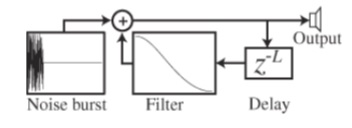
\includegraphics{res/ks_concept.jpg}
    \caption{Diagrama Conceptual del Modelo de Karplus-Strong}
    \label{fig:KS_model}
\end{figure}

La línea de retardo simula cómo los distintos armónicos de una nota recorren la línea, se atenúan y decaen en el tiempo. Se suele utilizar un filtro pasa-bajos para atenuar más rápidamente los armónicos de más altas frecuencias. Nótese que la longitud de la secuencia de entrada debe tener una longitud $L \in \mathbb{N}$.

La primera etapa de este modelo promedia dos muestras consecutivas. Este proceso puede describirse matemáticamente como la ecuación \eqref{eq:KS_avg}.

\begin{equation}
    Y_t = 0.5\times \left(Y_{t-L}+Y_{t-L-1}\right)
    \label{eq:KS_avg}
\end{equation}

Resulta que este promediamiento produce una onda que decae más lentamente en el tiempo. El onda generada por este algoritmo corresponde a un tono con período $L + 0.5$ muestras (que corresponde a una frecuencia de $f_s / (L+0.5)$) y suena más cercanamente al sonido de una cuerda punteada.

Independientemente de las condiciones iniciales del sistema, el espectro decaerá a un tono puro, y eventualmente, a una constante (el silencio). A pesar que el modelo de recurrencia no tiene entrada, es necesario especificar condiciones iniciales no nulas para iniciarlo. Por otro lado, para producir un sonido realista, se desea que el impulso inicial contenga muchos armónicos.
Esto se logra llenando el sistema con valores aleatorios al principio de cada nota generada. Dado que estas muestras aleatorias son repetidas periódicamente, no producen ruido.

Una manera de implementar esta aleatoriedad rápidamente es utilizando aleatoriedad de dos niveles, donde matemáticamente las condiciones iniciales están dadas por la expresión \eqref{eq:2_level_random}, donde $A$ será la amplitud de la onda.

\begin{equation}
    Y_t = 
    \begin{cases}
        +A  &   \text{probabilidad 0.5}\\
        -A  &   \text{probabilidad 0.5}
    \end{cases}
    \qquad  \text{para} -L\leq t \leq 0
    \label{eq:2_level_random}
\end{equation}

El modelo final del modelo para una cuerda percutida estará dado por el visto en la figura \ref{fig:ks_original}. $x(n)$ será la señal inicial de entrada, que en este caso será una señal de ruido de longitud de muestras $L$.

\begin{figure}[ht]
    \centering
    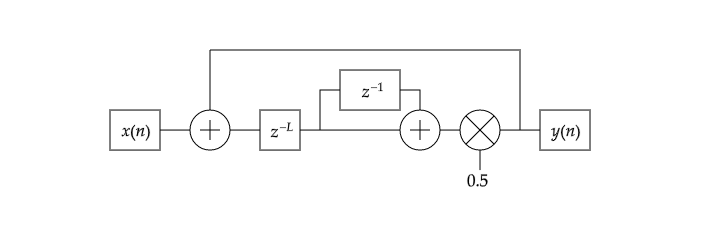
\includegraphics[width = \linewidth]{res/fig_ks.png}
    \caption{Modelo Original de Karplus Strong}
    \label{fig:ks_original}
\end{figure}

Existe una modificación donde además del proceso de promediación, se cambia el signo de la muestra aleatoriamente, como se ve en la figura \ref{fig:ks_drum}. Su comportamiento queda evidenciado en la expresión \eqref{eq:ks_drum}:

\begin{figure}[ht]
    \centering
    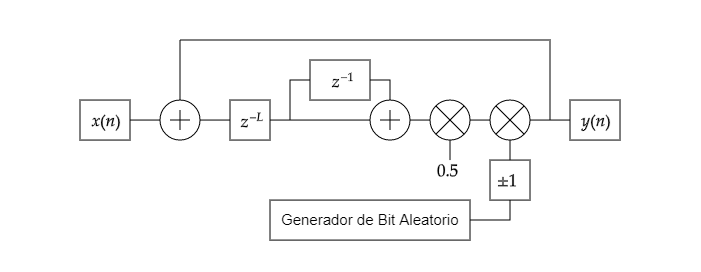
\includegraphics[width = \linewidth]{res/fig_ks_drum.png}
    \caption{Modelo Modificado de Karplus Strong para instrumentos de percusión}
    \label{fig:ks_drum}
\end{figure}

\begin{equation}
    Y_t = 
    \begin{cases}
        0.5\times \left(Y_{t-L}+Y_{t-L-1}\right) &   \text{probabilidad} \quad b \\
        -0.5\times \left(Y_{t-L}+Y_{t-L-1}\right) &   \text{probabilidad} \quad 1-b
    \end{cases}
    \label{eq:ks_drum}
\end{equation}

donde $b$ se le llama factor de mezcla. Cuando $b = 0.5$ se produce un sonido similar a un tambor. Cualquier valor intermedio producirá sonidos entre una cuerda o tambor. Cuando $b = 0$ la señal es negada cada $L + 0.5$ muestras, produciendo un sonido de ``botella percutida'' a altas frecuencias, y un sonido de harpa a bajas frecuencias.

Cuando $b=0.5$, la longitud de las muestras ya no controla el tono del sonido, ya que el sonido ya no es periódico. En lugar de eso, $L$ controla el tiempo de decaimiento del ruido de manera proporcional. Para estos, la señal de entrada puede simplemente ser una constante $A$, dado que el algoritmo mismo generará la aleatoriedad.

Limitando los valores de $b$ a $\left\{ 0;0.5;1\right\}$ será suficiente utilizar solo un bit para generar la aleatoriedad. Si se usaren otros valores será necesario utilizar un generador de números aleatorios más sofisticado.

\section{Transferencia del Modelo}

A partir del modelo de la figura \ref{fig:ks_original} se obtiene que la función transferencia estará dada por \eqref{eq:Hz_KS}

\begin{equation}
    H(z) = \frac{1/2\cdot (1+z^{-1})}{1-1/2\cdot z^{-L}(1+z^{-1})}= \frac{z+1}{2z^{L+1}-z-1}
    \label{eq:Hz_KS}
\end{equation}

Los polos pueden ser encontrados mediante la expresión $2z^{L+1}-z-1 = 0$ mientras que se encuentra el único cero en $z=-1$. Este corresponde a la frecuencia de Nyquist $f_s/2$.

Se pueden aproximar las raíces de $2z^{L+1}-z-1 = 0$ si la expresamos de la forma $2z^{L+1/2} = z^{1/2} + z^{-1/2}$. Reemplazando $z=a e^{j\omega}$ se obtiene:

\begin{equation}
    2 a^{L+1/2} e^{j\omega (L+1/2)} = a^{1/2}e^{j\omega/2} + a^{-1/2}e^{-j\omega/2}
\end{equation}

Aproximando $e^{j\omega}(L+1/2) \approx 1$ se despeja que $\omega = 2 \pi n / (L+1/2)$. Aproximando $2 a^{p+1/2}\approx 2 cos(\omega/2)$ se puede despejar la constante del tiempo de caída del n-ésimo armónico, siendo
\begin{equation}
    a=\left[cos\left( \frac{2 \pi n}{2L+1}\right)\right]^{1/(L+1/2)}
\end{equation}